
For the optimal solution, $\Phi_{residue}=9\cross10^{-15}$, we map out the surface this variable defines in solution space using two coordinate systems.
%----------------------------------------------------------------------------
%----------------------------------------------------------------------------
The region in solution space near the optimal solution shown in Figure \ref{solution 2 pulses} was mapped out by allowing the magnitude of $\Delta_{\alpha}$ and $A$ to vary by $\pm 50\%$. Figure \ref{delay amp} shows the resulting $\log(\Psi_{residue})$ surface.
%----------------------------------------------------------------------------
%----------------------------------------------------------------------------
The region in solution space near the optimal solution shown in Figure \ref{solution 2 pulses} was mapped out by allowing the magnitude of $A$ and $B$ to vary by $\pm 50\%$. Figure \ref{amp amp} shows the resulting $\log(\Psi_{residue})$ surface. Figures \ref{delay amp} and \ref{amp amp} show the robustness of the STIRAP process with regards to population transfer. The since the residue is less than $10^{-2}$ for most of the points (i.e. there is very little population left over in states 0 and 1) population transfer in nearly complete for relatively large detuning of certain pulse parameters (amplitude and delay). This means that even if there are fluctuations in these parameters, the targeted two color pathway will still result in nearly complete population transfer; thus the probability that the final target state releases a fluorescence photon is nearly independent of these types of fluctuations.
%----------------------------------------------------------------------------
%----------------------------------------------------------------------------
% delay_amp.tex
% by Troy Hix, March 2005
%----------------------------------------------------------------------------
\begin{figure}
\centering
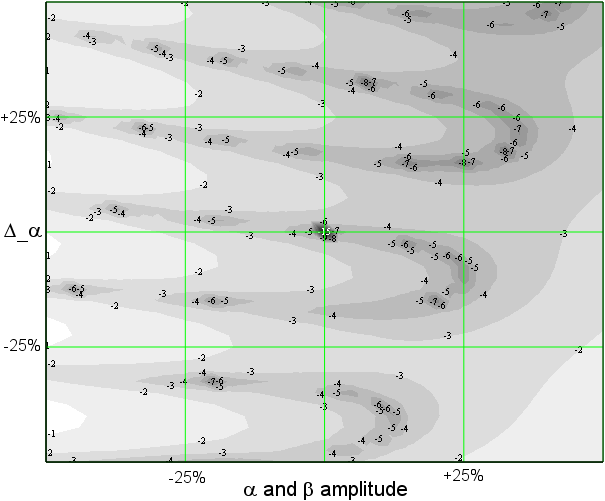
\includegraphics[width=4.00in]
{delay_amp/delay_amp.png}\\
\caption[$\log\left(\Phi_{residue}\right)$ dependence on scaling $\Delta_{\alpha}$ and $A$]{$\log\left(\Phi_{residue}\right)$ dependence on scaling $\Delta_{\alpha}$ and $A$. There are many local optima arranged in a repeating crescent shape. In general the local optima and the average height of the nearby surface decreases as $\Delta_{\alpha}$ and $A$ increase. There are $41^2$ evenly spaced points here.}
\label{delay amp}
\end{figure} 
%----------------------------------------------------------------------------

%----------------------------------------------------------------------------
%----------------------------------------------------------------------------
% amp_amp.tex
% by Troy Hix, March 2005
%----------------------------------------------------------------------------
\begin{figure}
\centering
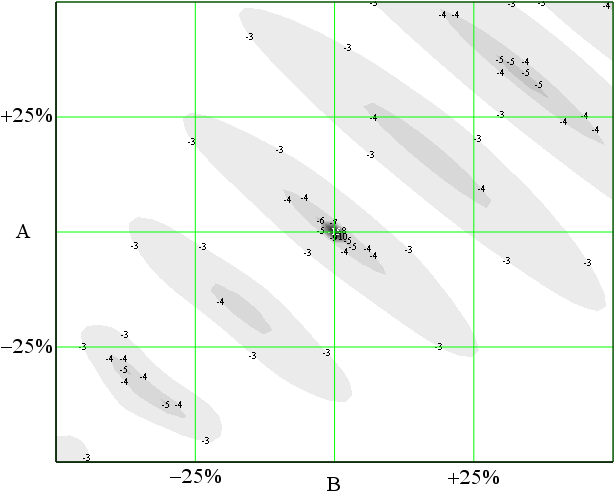
\includegraphics[width=4.00in]
{amp_amp/amp_amp.png}\\
\caption[$\Phi_{residue}$ dependence on scaling $A$ and $B$]{$\Phi_{residue}$ dependence on scaling $A$ and $B$. There are many local optima along the line defined by $A=B$. These optima improve as amplitudes $A$ and $B$ increase; and, in general, the surface slopes down as $A$ and $B$ increase. There are $41^2$ evenly spaced points here.}
\label{amp amp}
\end{figure} 
%----------------------------------------------------------------------------

%----------------------------------------------------------------------------
%----------------------------------------------------------------------------
